% ============================================================
% SECCIÓN 8 — Teorema de Green-Tao (5 min)
% ============================================================

% --- Diapositiva 1: El problema de densidad cero ---
\begin{frame}{Green-Tao: El Obstáculo}

    \begin{block}{Recordatorio — Szemerédi}
        Garantiza PA de cualquier longitud en conjuntos con
        $d(A) > 0$.
    \end{block}

    \vspace{0.3cm}

    Por el \textbf{Teorema de los Números Primos}:
    \[
        \pi(n) \sim \frac{n}{\ln n}
        \quad\Longrightarrow\quad
        d\bigl(\{p : p \text{ es primo}\}\bigr)
        = \lim_{n\to\infty}\frac{\pi(n)}{n} = 0
    \]

    \pause
    \vspace{0.3cm}

    \begin{alertblock}{Obstáculo}
        $d(\text{primos}) = 0 \;\Rightarrow\;$ \textbf{Szemerédi no aplica}.\\[4pt]
        ¿Contienen los primos progresiones aritméticas
        arbitrariamente largas?
    \end{alertblock}

    \pause
    \vspace{0.3cm}

    \begin{exampleblock}{Respuesta (Green y Tao, 2004)}
        \centering
        \textbf{¡Sí!} Los primos contienen PA de cualquier
        longitud finita $k$.
    \end{exampleblock}

\end{frame}


% --- Diapositiva 2: Ejemplos visuales ---
\begin{frame}{Ejemplos de PA en los Primos}

    \begin{columns}[T]

        \begin{column}{0.55\textwidth}
        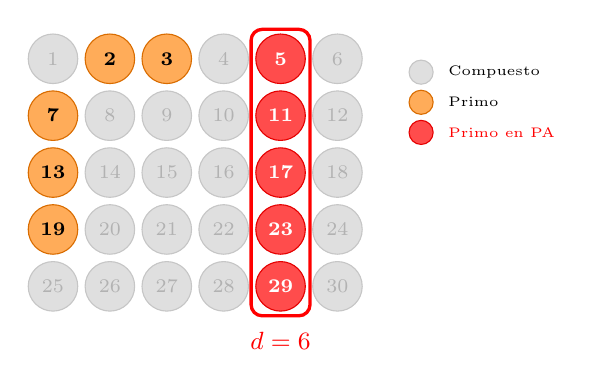
\begin{tikzpicture}[scale=0.85]
            % Números compuestos
            \foreach \n/\xi/\yi in {
                1/0/0, 4/3/0, 6/5/0,
                8/1/1, 9/2/1, 10/3/1, 12/5/1,
                14/1/2, 15/2/2, 16/3/2, 18/5/2,
                20/1/3, 21/2/3, 22/3/3, 24/5/3,
                25/0/4, 26/1/4, 27/2/4, 28/3/4, 30/5/4}{
                \filldraw[gray!25, draw=gray!45]
                    ({0.85*\xi},{-0.85*\yi}) circle (0.37cm);
                \node[text=gray!60, font=\scriptsize]
                    at ({0.85*\xi},{-0.85*\yi}) {\n};
            }
            % Primos normales
            \foreach \n/\xi/\yi in {2/1/0, 3/2/0, 7/0/1, 13/0/2, 19/0/3}{
                \filldraw[orange!65, draw=orange!85!black]
                    ({0.85*\xi},{-0.85*\yi}) circle (0.37cm);
                \node[text=black, font=\scriptsize\bfseries]
                    at ({0.85*\xi},{-0.85*\yi}) {\n};
            }
            % PA: 5,11,17,23,29 con d=6
            \foreach \n/\xi/\yi in {5/4/0, 11/4/1, 17/4/2, 23/4/3, 29/4/4}{
                \filldraw[red!70, draw=red!90!black]
                    ({0.85*\xi},{-0.85*\yi}) circle (0.37cm);
                \node[text=white, font=\scriptsize\bfseries]
                    at ({0.85*\xi},{-0.85*\yi}) {\n};
            }
            % Caja PA
            \draw[red, very thick, rounded corners=4pt]
                ({0.85*4-0.44}, 0.44) rectangle
                ({0.85*4+0.44}, {-0.85*4-0.44});
            \node[red, font=\small\bfseries]
                at ({0.85*4}, {-0.85*4-0.82}) {$d=6$};
            % Leyenda
            \filldraw[gray!25,   draw=gray!45]         (5.5,-0.20) circle (0.18cm);
            \node[font=\tiny, right=1pt] at (5.72,-0.20) {Compuesto};
            \filldraw[orange!65, draw=orange!85!black] (5.5,-0.65) circle (0.18cm);
            \node[font=\tiny, right=1pt] at (5.72,-0.65) {Primo};
            \filldraw[red!70,    draw=red!90!black]    (5.5,-1.10) circle (0.18cm);
            \node[font=\tiny, right=1pt, red] at (5.72,-1.10) {Primo en PA};
        \end{tikzpicture}
        \end{column}

        \begin{column}{0.42\textwidth}
            \textbf{Ejemplos concretos:}
            \begin{align*}
                k=3\colon &\quad 3,\;7,\;11 \\[3pt]
                k=5\colon &\quad 5,\;11,\;17,\;23,\;29 \\[3pt]
                k=10\colon &\quad 199,\;\ldots,\;2089
            \end{align*}

            \vspace{0.3cm}

            \begin{block}{Cuadro comparativo}
            {\footnotesize
            \begin{tabular}{ll}
                \hline
                VdW     & coloración $\to$ PA \\
                Szem.   & $d>0$ $\to$ PA \\
                G-T     & primos ($d=0$) $\to$ PA \\
                \hline
            \end{tabular}}
            \end{block}
        \end{column}

    \end{columns}

\end{frame}


% --- Diapositiva 3: Idea de la demostración ---
\begin{frame}{Idea de la Demostración de Green-Tao}

    \begin{columns}[T]

        \begin{column}{0.5\textwidth}
            \begin{block}{El problema}
                Los primos tienen densidad $0$, por lo que
                Szemerédi no aplica directamente.
            \end{block}

            \vspace{0.3cm}

            \textbf{Idea clave:} encontrar un conjunto \textit{casi
            primo} $B$ con:
            \begin{enumerate}
                \item $d(B) > 0$ dentro de $B$, los primos son
                      ``densos''.
                \item Los primos se comportan \textbf{pseudo-aleatoriamente}
                      dentro de $B$.
            \end{enumerate}
        \end{column}

        \begin{column}{0.46\textwidth}
            \begin{exampleblock}{Ingredientes}
                \begin{itemize}
                    \item Criba de Goldston-Pintz-Yildirim
                    \item Generalización de Szemerédi a\\
                          entornos pseudo-aleatorios
                    \item Teoría ergódica y análisis\\
                          de Fourier
                \end{itemize}
            \end{exampleblock}

            \vspace{0.3cm}

            \begin{alertblock}{Impacto}
                Premio Salem 2004 (Green)\\
                Medalla Fields 2006 (Tao)
            \end{alertblock}
        \end{column}

    \end{columns}

\end{frame}
